% chktex-file 13

\documentclass{article}
\usepackage{amsmath}
\usepackage[a4paper, top=0.75in, bottom=0.75in]{geometry}
\usepackage{enumitem}
\usepackage{graphicx}

\graphicspath{ {./images/} }

\title{Homework 2}
\author{David Robinson}
\date{}
\setlength{\parindent}{0pt}

\begin{document}

\maketitle

\subsection*{Problem 1: NFA Properties}
The following NFA recognizes a language where the string contains the number 1. If the accept and non-accept states were swapped where $q_0$ becomes an accept state and $q_1$ is no longer an accept state, the resulting NFA does not recognize a language where the string does not contain the number 1 as the string ``1'' has a path with $q_0$.

\begin{center}
    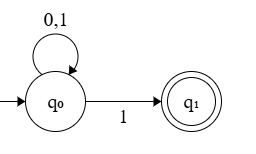
\includegraphics[scale=0.65]{nfa.png}
\end{center}

Yes, the class of language recognized by NFAs is closed by complement because DFAs are closed under complement, and every NFA has an equivalent DFA. Since an NFA can be converted into a DFA that recognizes the same language, the complement of that DFA can be converted back into an NFA.

\subsection*{Problem 2: Regular Expression}

\[/\#{({(a\cup b\cup /)}^*{(\#^*(a\cup b))}^*)}^* \#^*\#/\]

\subsection*{Problem 3: The Regular Property}

\begin{itemize}
    \item Since $A$ and $B$ are regular languages, they can be recognized by finite automatas, $M_A$ and $M_B$, respectively. A new finite automaton can be used to interleave the transitions in $M_A$ and $M_B$ by alternating between input symbols from $A$ and $B$. Through a product construction, the finite automaton can track both $M_A$ and $M_B$ states and the resulting language is regular.
    \item Since $A$ and $B$ are regular languages, they can be recognized by finite automatas, $M_A$ and $M_B$, respectively. An NFA can be used to recognize the shuffle of $A$ and $B$ by providing transitions with the next possible symbols from $A$ and $B$. Since NFAs are equivalent to DFAs, the new language is regular.
\end{itemize}

\subsection*{Problem 4: Parameterized Regularity}

An NFA that represents all strings $\Sigma^*\mathbf{a}\Sigma^{k-1}$ can be constructed with a sequence of $k+1$ states. The starting state should have a self-loop for all symbols in the alphabet to allow all symbols preceding the $\mathbf{a}$. This state will have a transition on $\mathbf{a}$ to the next state. The next $k-1$ states will all have transitions on $\Sigma$ to represent each of the $k-1$ symbols after $\mathbf{a}$.
\vspace{1em}

The following NFA represents all strings $\Sigma^*\mathbf{a}\Sigma^{k-1}$ for $k=3$ with $k+1=4$ states.

\begin{center}
    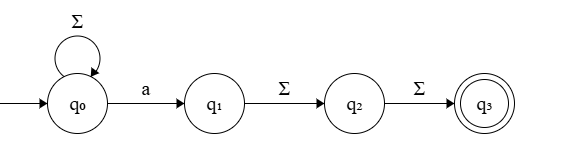
\includegraphics[scale=0.65]{nfa2.png}
\end{center}

\pagebreak
\subsection*{Problem 5: Irregularity}

\begin{enumerate}[label=\Alph*.]
    \item $L=\{sss\: |\text{ $s$ is any string over }\Sigma\}$ with $\Sigma=\{\mathbf{a}, \mathbf{b}\}$
    
    Let $s=a^p$, the corresponding string in $L$ is $w=a^p a^p a^p$, and $w=xyz$ with $|xy|\leq p$. Since the first $p$ symbols are in the first $s$ of $w$, pumping $y$ breaks the triple repetition in $L$ and allows other number of repetitions of $s$. The resulting string may not be in the form $sss$ for some $s$. The language is not regular because it is not closed under the Pumping Lemma.
    \item $L=\{x=y+z\:|\text{ $x$, $y$, and $z$ are binary integers}\}$ with $\Sigma=\{\mathbf{0},\mathbf{1},\mathbf{+},\mathbf{=}\}$
    
    Let $s$ be the string $1^p 0=1^p +1^p$ and $s=xyz$ with $|xy|\leq p$. Since the first $p$ symbols are all $1$'s from the sum, $y$ consists of only $1$'s from the sum. Pumping $y$ increases the left-hand sum while the addends remain the same, resulting in an invalid equation. The language is not regular because it is not closed under the Pumping Lemma.
    \item $L=\{\mathbf{a}^n\mathbf{b}^m\mathbf{a}^n\:|\text{ $m$ and $n$ are non-negative integers}\}$ with $\Sigma=\{\mathbf{a}, \mathbf{b}\}$

    Let $s=a^p b^m a^p$ and $s=xyz$ with $|xy|\leq p$. Since the first $p$ symbols are $a$'s, $xy$ only consists of $a$'s and therefore, $y$ only consists of $a$'s. Pumping $y$ increases the number of leading $a$'s but not the number of trailing $a$'s so the new string does not preserve the original pattern of $a^n b^m a^n$. The language is not regular because it is not closed under the Pumping Lemma.
    \item $L=\{s\:|\text{ $s$ is a string over $\Sigma$ that is not a palindrome}\}$ with $\Sigma=\{\mathbf{a}, \mathbf{b}\}$
    
    Since the language of palindromes has already been proven to be not regular (part C) and non-regular languages are closed under complement, the language of non-palindromes is not regular.
\end{enumerate}

\end{document}